%package list
\documentclass{article}
\usepackage[top=3cm, bottom=3cm, outer=3cm, inner=3cm]{geometry}
\usepackage{graphicx}
\usepackage{url}
\usepackage{hyperref}
\usepackage{array}
\usepackage{natbib}
\usepackage{pdfpages}
\usepackage{multirow}
\usepackage[normalem]{ulem}
\useunder{\uline}{\ul}{}
\usepackage{xcolor}
\usepackage{listings}

\newcolumntype{x}[1]{>{\centering\arraybackslash\hspace{0pt}}p{#1}}
\usepackage{caption}
\usepackage{subcaption}
\usepackage{float}

\newcolumntype{M}[1]{>{\centering\arraybackslash}m{#1}}
\newcolumntype{N}{@{}m{0pt}@{}}

%%%%%%%%%%%%%%%%%%%%%%%%%%%%%%%%%%%%%%%%%%%%%%%%%%%%%%%%%%%%%%%%%%%%%%%%%%%%
%%%%%%%%%%%%%%%%%%%%%%%%%%%%%%%%%%%%%%%%%%%%%%%%%%%%%%%%%%%%%%%%%%%%%%%%%%%%
\newcommand{\itemEmail}{jgordillome@unsa.edu.pe}
\newcommand{\itemStudent}{Gordillo Mendoza Jose Alonzo}
\newcommand{\itemCourse}{Desarrollo en Nuevas Plataformas}
\newcommand{\itemSemester}{IX (noveno)}
\newcommand{\itemUniversity}{Universidad Nacional de San Agustín de Arequipa}
\newcommand{\itemFaculty}{Facultad de Ingeniería de Producción y Servicios}
\newcommand{\itemDepartment}{Departamento Académico de Ingeniería de Sistemas e Informática}
\newcommand{\itemSchool}{Escuela Profesional de Ingeniería de Sistemas}
\newcommand{\itemAcademic}{2026 - A}
\newcommand{\itemPracticeNumber}{09}
\newcommand{\itemPracticeTitle}{APIs REST en Compose: Consumo de Datos}
\newcommand{\itemTheme}{Sincronización de Datos Offline-First y Notificaciones Push}
\newcommand{\itemDocente}{MSc. Norman Patrick Harvey Arce}
\newcommand{\itemSubmitDate}{29/06/2026}
\newcommand{\itemSubmitTime}{23:59}
\newcommand{\itemReportDate}{13 de julio de 2026}
\newcommand{\itemRepoUrl}{https://github.com/JoseGordilloMendoza/apiApp.git}
%%%%%%%%%%%%%%%%%%%%%%%%%%%%%%%%%%%%%%%%%%%%%%%%%%%%%%%%%%%%%%%%%%%%%%%%%%%%
%%%%%%%%%%%%%%%%%%%%%%%%%%%%%%%%%%%%%%%%%%%%%%%%%%%%%%%%%%%%%%%%%%%%%%%%%%%%

\usepackage[english,spanish]{babel}
\usepackage[utf8]{inputenc}
\usepackage[T1]{fontenc}
\AtBeginDocument{\selectlanguage{spanish}}
\renewcommand{\figurename}{Figura}
\renewcommand{\refname}{Referencias}
\AtBeginDocument{%
	\renewcommand\tablename{Tabla}
}

\usepackage{fancyhdr}
\pagestyle{fancy}
\fancyhf{}
\setlength{\headheight}{30pt}
\renewcommand{\headrulewidth}{1pt}
\renewcommand{\footrulewidth}{1pt}
\fancyhead[L]{\raisebox{-0.2\height}{
\includegraphics[width=3cm]{img/logo_episunsa.png}}}
\fancyhead[C]{\fontsize{7}{7}\selectfont	\itemUniversity \\ \itemFaculty \\ \itemDepartment \\ \itemSchool \\ \textbf{\itemCourse}}
\fancyhead[R]{\raisebox{-0.2\height}{
\includegraphics[width=1.2cm]{img/logo_abet.png}}}
\fancyfoot[L]{Estudiante \itemStudent}
\fancyfoot[C]{\itemCourse}
\fancyfoot[R]{Página \thepage}

% Configuracion general de listados de codigo
\usepackage{color, colortbl}
\definecolor{dkgreen}{rgb}{0,0.6,0}
\definecolor{gray}{rgb}{0.5,0.5,0.5}
\definecolor{mauve}{rgb}{0.58,0,0.82}
\definecolor{codebackground}{rgb}{0.95, 0.95, 0.92}
\definecolor{tablebackground}{rgb}{0.8, 0, 0}

% Definicion de lenguaje Kotlin para listings (no viene incluido por defecto)
\lstdefinelanguage{Kotlin}{
	comment=[l]{//},
	commentstyle={\color{gray}\ttfamily},
	emphstyle={\color{orange}},
	identifierstyle=\color{black},
	keywords={abstract, actual, annotation, as, break, by, catch, class, companion, const, constructor, continue, crossinline, data, do, dynamic, else, enum, expect, external, false, final, finally, for, fun, get, if, import, in, infix, inline, inner, interface, internal, is, lateinit, noinline, null, object, open, operator, out, override, package, private, protected, public, reified, return, sealed, set, super, suspend, tailrec, this, throw, true, try, typealias, val, var, vararg, when, where, while},
	keywordstyle={\color{blue}\bfseries},
	morecomment=[s]{/*}{*/},
	morestring=[b]",
	ndkeywords={Array, Byte, Double, Float, Boolean, Int, Integer, Iterable, Long, Runnable, Short, String, Unit, Flow, StateFlow, Result},
	ndkeywordstyle={\color{purple}\bfseries},
	sensitive=true,
	stringstyle={\color{mauve}},
}

\lstset{frame=tb,
	language=bash,
	aboveskip=3mm,
	belowskip=3mm,
	showstringspaces=false,
	columns=flexible,
	basicstyle={\small\ttfamily},
	numbers=none,
	numberstyle=\tiny\color{gray},
	keywordstyle=\color{blue},
	commentstyle=\color{dkgreen},
	stringstyle=\color{mauve},
	breaklines=true,
	breakatwhitespace=true,
	tabsize=3,
	backgroundcolor=\color{codebackground},
}

\begin{document}

	\vspace*{10px}

	\begin{center}
		\fontsize{17}{17} \textbf{ Informe de Laboratorio \itemPracticeNumber}
	\end{center}
	\centerline{\textbf{\Large Título: \itemPracticeTitle}}
	\centerline{\large Tema: \itemTheme}

	\begin{flushright}
		\begin{tabular}{|M{2.5cm}|N|}
			\hline
			\rowcolor{tablebackground}
			\color{white} \textbf{Nota}  \\
			\hline
			     \\[30pt]
			\hline
		\end{tabular}
	\end{flushright}

	\begin{table}[H]
		\begin{tabular}{|x{4.7cm}|x{4.8cm}|x{4.8cm}|}
			\hline
			\rowcolor{tablebackground}
			\color{white} \textbf{Estudiante} & \color{white}\textbf{Escuela}  & \color{white}\textbf{Asignatura}   \\
			\hline
			{\itemStudent \par \itemEmail} & \itemSchool & {\itemCourse \par Semestre: \itemSemester}     \\
			\hline
		\end{tabular}
	\end{table}

	\begin{table}[H]
		\begin{tabular}{|x{4.7cm}|x{4.8cm}|x{4.8cm}|}
			\hline
			\rowcolor{tablebackground}
			\color{white}\textbf{Nro. de práctica} & \color{white}\textbf{Título de la práctica}  & \color{white}\textbf{Docente}   \\
			\hline
			\itemPracticeNumber & \itemPracticeTitle & \itemDocente   \\
			\hline
		\end{tabular}
	\end{table}

	\begin{table}[H]
		\begin{tabular}{|x{4.7cm}|x{4.8cm}|x{4.8cm}|}
			\hline
			\rowcolor{tablebackground}
			\color{white}\textbf{Año lectivo} & \color{white}\textbf{Semestre}  & \color{white}\textbf{Fecha y hora de presentación}   \\
			\hline
			\itemAcademic & \itemSemester &  \itemSubmitDate \ -- \ \itemSubmitTime \ hrs  \\
			\hline
		\end{tabular}
	\end{table}

	\begin{center}
		\small Fecha de elaboración del presente informe: \itemReportDate
	\end{center}

	\section{Tarea}
	El objetivo de esta práctica es extender una aplicación Android existente que consume una API REST (usando Retrofit y Jetpack Compose) para convertirla en una aplicación \textbf{Offline-First}, cumpliendo los siguientes objetivos:
	\begin{itemize}
		\item[a.] Funcionar sin conexión a Internet.
		\item[b.] Persistir los datos localmente en el dispositivo.
		\item[c.] Sincronizarse automáticamente con la API cuando se recupera la conexión de red.
		\item[d.] Mantener consistencia entre la interfaz de usuario (UI), el cache local y la API remota.
	\end{itemize}
	Adicionalmente, se debía incorporar \textbf{notificaciones push} que informen al usuario sobre eventos relevantes del ciclo de sincronización.

	\section{URL de Repositorio GitHub}
	\begin{itemize}
		\item URL del repositorio en GitHub donde se aloja el código fuente de la práctica.
		\item \url{\itemRepoUrl}
	\end{itemize}

	\section{Análisis de la aplicación base}
	Antes de iniciar la práctica se analizó el estado del proyecto entregado (\texttt{apiapp}), una app Android nativa en Kotlin con Jetpack Compose siguiendo el patrón MVVM. Se encontró lo siguiente:
	\begin{itemize}
		\item Consumo de red con Retrofit + Gson contra un único endpoint GET de \texttt{JSONPlaceholder} (\texttt{/todos}), paginado manualmente con los parámetros \texttt{\_start} y \texttt{\_limit}.
		\item Un \texttt{TodoRepository} que solo envolvía la respuesta de red en un \texttt{Result<>}, sin ningún tipo de persistencia.
		\item Un \texttt{UiState} (Loading/Success/Error) alimentado directamente por la respuesta de red: sin conexión, la aplicación simplemente fallaba.
		\item Inyección de dependencias manual (un \texttt{object NetworkModule} y un \texttt{ViewModelProvider.Factory} anónimo en \texttt{MainActivity}).
		\item Ausencia total de Room, WorkManager, \texttt{ConnectivityManager} y cualquier mecanismo de notificaciones.
	\end{itemize}
	Esta base era, en esencia, un ejemplo de solo lectura sin ningún mecanismo de resiliencia ante la falta de red, lo que la convertía en un punto de partida adecuado para demostrar el valor de una arquitectura Offline-First.

	\section{Pivote de API}
	La API original, \texttt{JSONPlaceholder}, es una API de pruebas de solo lectura: sus endpoints de escritura (POST/PUT/DELETE) responden con un código 200 simulado pero \textbf{no persisten nada en el servidor}. Además, su dataset de tareas (\textit{todos}) es genérico y no tiene ningún atractivo visual (no trae imágenes ni datos ricos), lo que limitaba severamente la posibilidad de demostrar visualmente el cacheo offline.

	Por este motivo se decidió \textbf{pivotear} el consumo de datos hacia la \href{https://rickandmortyapi.com/documentation}{Rick and Morty API}, una API pública, gratuita y sin autenticación que expone personajes de la serie con imagen, estado (\textit{Alive/Dead/unknown}), especie, género, ubicación de origen y ubicación actual. Las razones concretas del pivote fueron:
	\begin{itemize}
		\item El dataset es \textbf{relativamente estático} (los personajes no cambian de un minuto a otro), lo cual es ideal para demostrar un cache offline sin que el usuario note "datos desactualizados" de forma confusa.
		\item Trae \textbf{imágenes}, lo que permite demostrar también el cacheo de Coil en disco además del cacheo de datos en Room.
		\item Mantiene el mismo modelo de paginación por número de página que ya usaba la app original, minimizando el costo de migración de la capa de red.
	\end{itemize}
	Este pivote implicó reemplazar el modelo de dominio \texttt{Todo} por \texttt{Character}, el \texttt{ApiService} y sus DTOs, y renombrar las pantallas de \texttt{TodoScreen}/\texttt{TodoViewModel} a \texttt{CharacterScreen}/\texttt{CharacterViewModel}, conservando la arquitectura general (MVVM + Repository) del proyecto original.

	\section{Arquitectura Offline-First}
	La arquitectura implementada sigue el patrón \textbf{Single Source of Truth (SSOT)}: la interfaz de usuario nunca observa la respuesta de red directamente, sino un \texttt{Flow} expuesto por Room. La capa de red solo se usa para \textit{alimentar} la base de datos local; la UI reacciona exclusivamente a los cambios en Room.

	\begin{lstlisting}[language=bash,caption={Flujo de datos de la arquitectura Offline-First}]
UI (Compose) <-> ViewModel <-> Repository <-> Room (SSOT, Flow)
                                    |
                            Retrofit (red) <-> SyncWorker (WorkManager)
                                    |
                         ConnectivityObserver (NetworkCallback)
	\end{lstlisting}

	A continuación se detalla cómo se cumple cada uno de los cuatro objetivos del laboratorio, con el código concreto que lo implementa.

	\subsection{Objetivo a) Funcionar sin conexión a Internet}
	Se implementó un \texttt{ConnectivityObserver} que envuelve un \texttt{ConnectivityManager.NetworkCallback} en un \texttt{callbackFlow}, exponiendo el estado de conexión como un \texttt{Flow<Boolean>} reactivo que la UI colecta como \texttt{StateFlow}.
	\begin{lstlisting}[language=Kotlin,caption={NetworkConnectivityObserver.kt -- deteccion reactiva de conectividad}]
override val isConnected: Flow<Boolean> = callbackFlow {
    val callback = object : ConnectivityManager.NetworkCallback() {
        override fun onAvailable(network: Network) { trySend(hasInternet()) }
        override fun onLost(network: Network) { trySend(hasInternet()) }
        override fun onCapabilitiesChanged(
            network: Network, capabilities: NetworkCapabilities
        ) { trySend(hasInternet()) }
    }
    val request = NetworkRequest.Builder()
        .addCapability(NetworkCapabilities.NET_CAPABILITY_INTERNET)
        .build()
    connectivityManager.registerNetworkCallback(request, callback)
    trySend(hasInternet())
    awaitClose { connectivityManager.unregisterNetworkCallback(callback) }
}.distinctUntilChanged()
	\end{lstlisting}
	Cuando no hay red, el \texttt{ViewModel} sigue leyendo de Room con normalidad: la lista de personajes se sigue mostrando con los últimos datos guardados, y la UI muestra un banner de aviso ("Sin conexión: mostrando datos guardados localmente") junto a un indicador de estado (punto rojo/verde) siempre visible.

	\subsection{Objetivo b) Persistir localmente}
	Se incorporó \textbf{Room} como motor de persistencia. La entidad \texttt{CharacterEntity} guarda, además de los datos del personaje, metadatos propios de la app (página de origen, orden de lista y si es favorito), y el DAO expone tanto operaciones reactivas como de una sola vez:
	\begin{lstlisting}[language=Kotlin,caption={CharacterEntity.kt}]
@Entity(tableName = "characters")
data class CharacterEntity(
    @PrimaryKey val id: Int,
    val name: String,
    val status: String,
    val species: String,
    val gender: String,
    val imageUrl: String,
    val locationName: String,
    val originName: String,
    val episodeCount: Int,
    val page: Int,
    val sortOrder: Int,
    val isFavorite: Boolean
)
	\end{lstlisting}
	\begin{lstlisting}[language=Kotlin,caption={CharacterDao.kt}]
@Dao
interface CharacterDao {
    @Query("SELECT * FROM characters ORDER BY sortOrder ASC")
    fun observeCharacters(): Flow<List<CharacterEntity>>

    @Upsert
    suspend fun upsertAll(characters: List<CharacterEntity>)

    @Query("SELECT COUNT(*) FROM characters")
    suspend fun count(): Int

    @Query("SELECT MAX(page) FROM characters")
    suspend fun getLastCachedPage(): Int?
}
	\end{lstlisting}
	Room persiste los datos en un archivo SQLite (\texttt{apiapp.db}) que sobrevive tanto al cierre de la app como a reinicios en frío sin conexión: al abrir la app sin red, \texttt{observeCharacters()} emite inmediatamente el último estado guardado.

	\subsection{Objetivo c) Sincronizarse automáticamente cuando haya red}
	La sincronización automática ocurre por dos vías complementarias:
	\begin{enumerate}
		\item \textbf{Reactiva}: el \texttt{ViewModel} colecta \texttt{isConnected} y detecta transiciones de \textit{offline} a \textit{online}, disparando una resincronización inmediata.
		\item \textbf{Programada}: un \texttt{SyncWorker} de WorkManager corre cada 15 minutos con la restricción \texttt{NetworkType.CONNECTED}, como respaldo cuando la app está en segundo plano.
	\end{enumerate}
	\begin{lstlisting}[language=Kotlin,caption={CharacterViewModel.kt -- deteccion de reconexion y resincronizacion}]
private fun observeConnectivity() {
    viewModelScope.launch {
        isConnected.collect { connected ->
            val previous = previousConnected
            if (previous != null && previous != connected) {
                if (connected) {
                    val previousCount = repository.characters.first().size
                    repository.refreshCachedPages().onSuccess { newTotal ->
                        notificationHelper.notifySyncComplete(
                            newItemsFound = newTotal > previousCount
                        )
                    }
                } else {
                    notificationHelper.notifyDisconnected()
                }
            }
            previousConnected = connected
        }
    }
}
	\end{lstlisting}
	\begin{lstlisting}[language=Kotlin,caption={SyncWorker.kt -- sincronizacion periodica en segundo plano}]
@HiltWorker
class SyncWorker @AssistedInject constructor(
    @Assisted context: Context,
    @Assisted params: WorkerParameters,
    private val repository: CharacterRepository,
    private val notificationHelper: NotificationHelper
) : CoroutineWorker(context, params) {

    override suspend fun doWork(): Result {
        val previousCount = repository.characters.first().size
        return repository.refreshCachedPages().fold(
            onSuccess = { newTotal ->
                if (newTotal > previousCount) {
                    notificationHelper.notifySyncComplete(newItemsFound = true)
                }
                Result.success()
            },
            onFailure = { Result.retry() }
        )
    }
}
	\end{lstlisting}
	Un detalle importante detectado y corregido durante las pruebas: como \texttt{@Upsert} sobrescribe la fila completa, un \textit{refresh} ingenuo borraría el estado de favorito local en cada sincronización. Por ello, antes de mapear la respuesta de red a entidades, el repositorio consulta los IDs marcados como favoritos y los preserva:
	\begin{lstlisting}[language=Kotlin,caption={CharacterRepository.kt -- preservacion de estado local al sincronizar}]
suspend fun refresh(page: Int): Result<Boolean> = try {
    val response = api.getCharacters(page)
    val favoriteIds = dao.getFavoriteIds().toSet()
    val startOrder = (page - 1) * PAGE_SIZE
    val entities = response.results.mapIndexed { index, dto ->
        dto.toEntity(page = page, sortOrder = startOrder + index,
            isFavorite = dto.id in favoriteIds)
    }
    dao.upsertAll(entities)
    markSynced()
    Result.success(response.info.next != null)
} catch (e: Exception) {
    Result.failure(e)
}
	\end{lstlisting}
	Adicionalmente, se creó una tabla \texttt{sync\_meta} con una única fila que guarda el timestamp del último sync exitoso (\texttt{markSynced()}), usada para mostrar en la UI "Sync: hace X min" incluso tras un arranque en frío sin conexión.

	\subsection{Objetivo d) Consistencia entre UI, cache local y API}
	El \texttt{CharacterRepository} expone un único \texttt{Flow<List<Character>>} derivado de Room, que es la \textbf{única fuente de verdad} tanto para la lista principal como para la pantalla de detalle. El \texttt{ViewModel} combina ese flujo con los estados de carga/error/filtros mediante \texttt{combine()}, garantizando que la UI siempre refleje exactamente lo que hay en la base de datos local:
	\begin{lstlisting}[language=Kotlin,caption={CharacterRepository.kt -- Room como Single Source of Truth}]
val characters: Flow<List<Character>> =
    dao.observeCharacters().map { entities -> entities.map { it.toDomain() } }
	\end{lstlisting}
	\begin{lstlisting}[language=Kotlin,caption={CharacterViewModel.kt -- combinacion reactiva de cache + filtros}]
val uiState: StateFlow<UiState> = combine(
    repository.characters,
    _isLoading,
    _errorMessage,
    _hasMore,
    filters
) { characters, isLoading, error, hasMore, filters ->
    val filtered = characters.filter { character ->
        (filters.query.isBlank() ||
            character.name.contains(filters.query, ignoreCase = true)) &&
        (filters.status.apiValue == null ||
            character.status.equals(filters.status.apiValue, ignoreCase = true)) &&
        (!filters.favoritesOnly || character.isFavorite)
    }
    when {
        characters.isEmpty() && error != null -> UiState.Error(error)
        characters.isEmpty() && isLoading -> UiState.Loading
        else -> UiState.Success(filtered, hasMore, isLoading && characters.isNotEmpty())
    }
}.stateIn(viewModelScope, SharingStarted.WhileSubscribed(5000), UiState.Loading)
	\end{lstlisting}
	Gracias a este diseño, una acción como marcar un personaje como favorito se refleja instantáneamente en la lista, en el filtro de favoritos y en la pantalla de detalle, sin necesidad de recargar nada manualmente: los tres se limitan a observar la misma fuente.

	\section{Notificaciones Push}
	Dado que la aplicación no cuenta con un backend propio (se consume una API pública de terceros de solo lectura efectiva), no es posible disparar \textbf{push remoto} real vía Firebase Cloud Messaging, ya que este requiere un servidor que emita los mensajes a través del Firebase Admin SDK. Se optó, en su lugar, por \textbf{notificaciones locales} generadas por el propio dispositivo en respuesta a eventos de conectividad, usando \texttt{NotificationCompat} sobre un canal de notificaciones dedicado (requerido desde Android 8) y solicitando el permiso en tiempo de ejecución \texttt{POST\_NOTIFICATIONS} (requerido desde Android 13).
	\begin{lstlisting}[language=Kotlin,caption={NotificationHelper.kt -- canal y disparo de notificaciones locales}]
@Singleton
class NotificationHelper @Inject constructor(
    @ApplicationContext private val context: Context
) {
    fun createChannel() {
        if (Build.VERSION.SDK_INT < Build.VERSION_CODES.O) return
        val channel = NotificationChannel(
            CHANNEL_ID, "Sincronización", NotificationManager.IMPORTANCE_DEFAULT
        ).apply { description = "Avisos sobre la sincronización de datos offline" }
        context.getSystemService(NotificationManager::class.java)
            ?.createNotificationChannel(channel)
    }

    fun notifySyncComplete(newItemsFound: Boolean) {
        val title = if (newItemsFound) "Nuevos personajes disponibles" else "Conexión restaurada"
        val text = if (newItemsFound) "Se sincronizaron nuevos personajes para verlos sin conexión"
            else "Tus datos guardados están actualizados"
        notify(title, text, NotificationCompat.PRIORITY_DEFAULT)
    }

    fun notifyDisconnected() {
        notify("Sin conexión", "Trabajando con los datos guardados localmente",
            NotificationCompat.PRIORITY_LOW)
    }

    private fun notify(title: String, text: String, priority: Int) {
        if (Build.VERSION.SDK_INT >= Build.VERSION_CODES.TIRAMISU &&
            ActivityCompat.checkSelfPermission(context, Manifest.permission.POST_NOTIFICATIONS)
                != PackageManager.PERMISSION_GRANTED
        ) return

        val notification = NotificationCompat.Builder(context, CHANNEL_ID)
            .setSmallIcon(R.drawable.ic_sync_notification)
            .setContentTitle(title)
            .setContentText(text)
            .setPriority(priority)
            .setAutoCancel(true)
            .build()
        NotificationManagerCompat.from(context).notify(NOTIFICATION_ID, notification)
    }

    companion object {
        const val CHANNEL_ID = "sync_channel"
        private const val NOTIFICATION_ID = 1001
    }
}
	\end{lstlisting}
	Se implementaron dos disparadores distintos, cubriendo ambos sentidos del cambio de red:
	\begin{itemize}
		\item \textbf{Reconexión}: "Conexión restaurada -- Tus datos guardados están actualizados" (o "Nuevos personajes disponibles" si el sync trajo datos nuevos).
		\item \textbf{Pérdida de conexión}: "Sin conexión -- Trabajando con los datos guardados localmente".
	\end{itemize}
	Esto demuestra que el sistema reacciona activamente a ambos sentidos de la transición de red, no solo al reconectar.

	\section{Estructura del proyecto}
	La distribución final de paquetes en \texttt{app/src/main/java/com/example/apiapp} quedó organizada por capas siguiendo el patrón MVVM + Repository:
	\begin{lstlisting}[language=bash,caption={Estructura de paquetes de la aplicacion}]
apiapp/
  ApiApp.kt                     (Application, Hilt + WorkManager)
  MainActivity.kt
  data/
    connectivity/
      ConnectivityObserver.kt
      NetworkConnectivityObserver.kt
    local/                      (Room: entities, DAOs, migraciones)
      AppDatabase.kt
      CharacterEntity.kt / CharacterDao.kt
      SyncMetaEntity.kt / SyncMetaDao.kt
      Migrations.kt
    model/
      Character.kt
    network/                    (Retrofit + DTOs)
      RickAndMortyApiService.kt
      dto/CharacterDto.kt
    repository/
      CharacterRepository.kt    (Single Source of Truth)
    sync/                       (WorkManager)
      SyncWorker.kt / SyncScheduler.kt
  di/                           (Modulos Hilt)
    NetworkModule.kt / DatabaseModule.kt / ConnectivityModule.kt
  notifications/
    NotificationHelper.kt
  ui/
    CharacterScreen.kt / CharacterDetailScreen.kt
    CharacterViewModel.kt / UiState.kt / StatusFilter.kt
	\end{lstlisting}

	\section{Ejecución}
	A continuación se muestra evidencia capturada directamente de la app corriendo sobre un emulador Android (Pixel 9 Pro, API 36), demostrando cada uno de los objetivos del laboratorio.

	\begin{figure}[H]
		\centering
		\begin{subfigure}[t]{0.42\textwidth}
			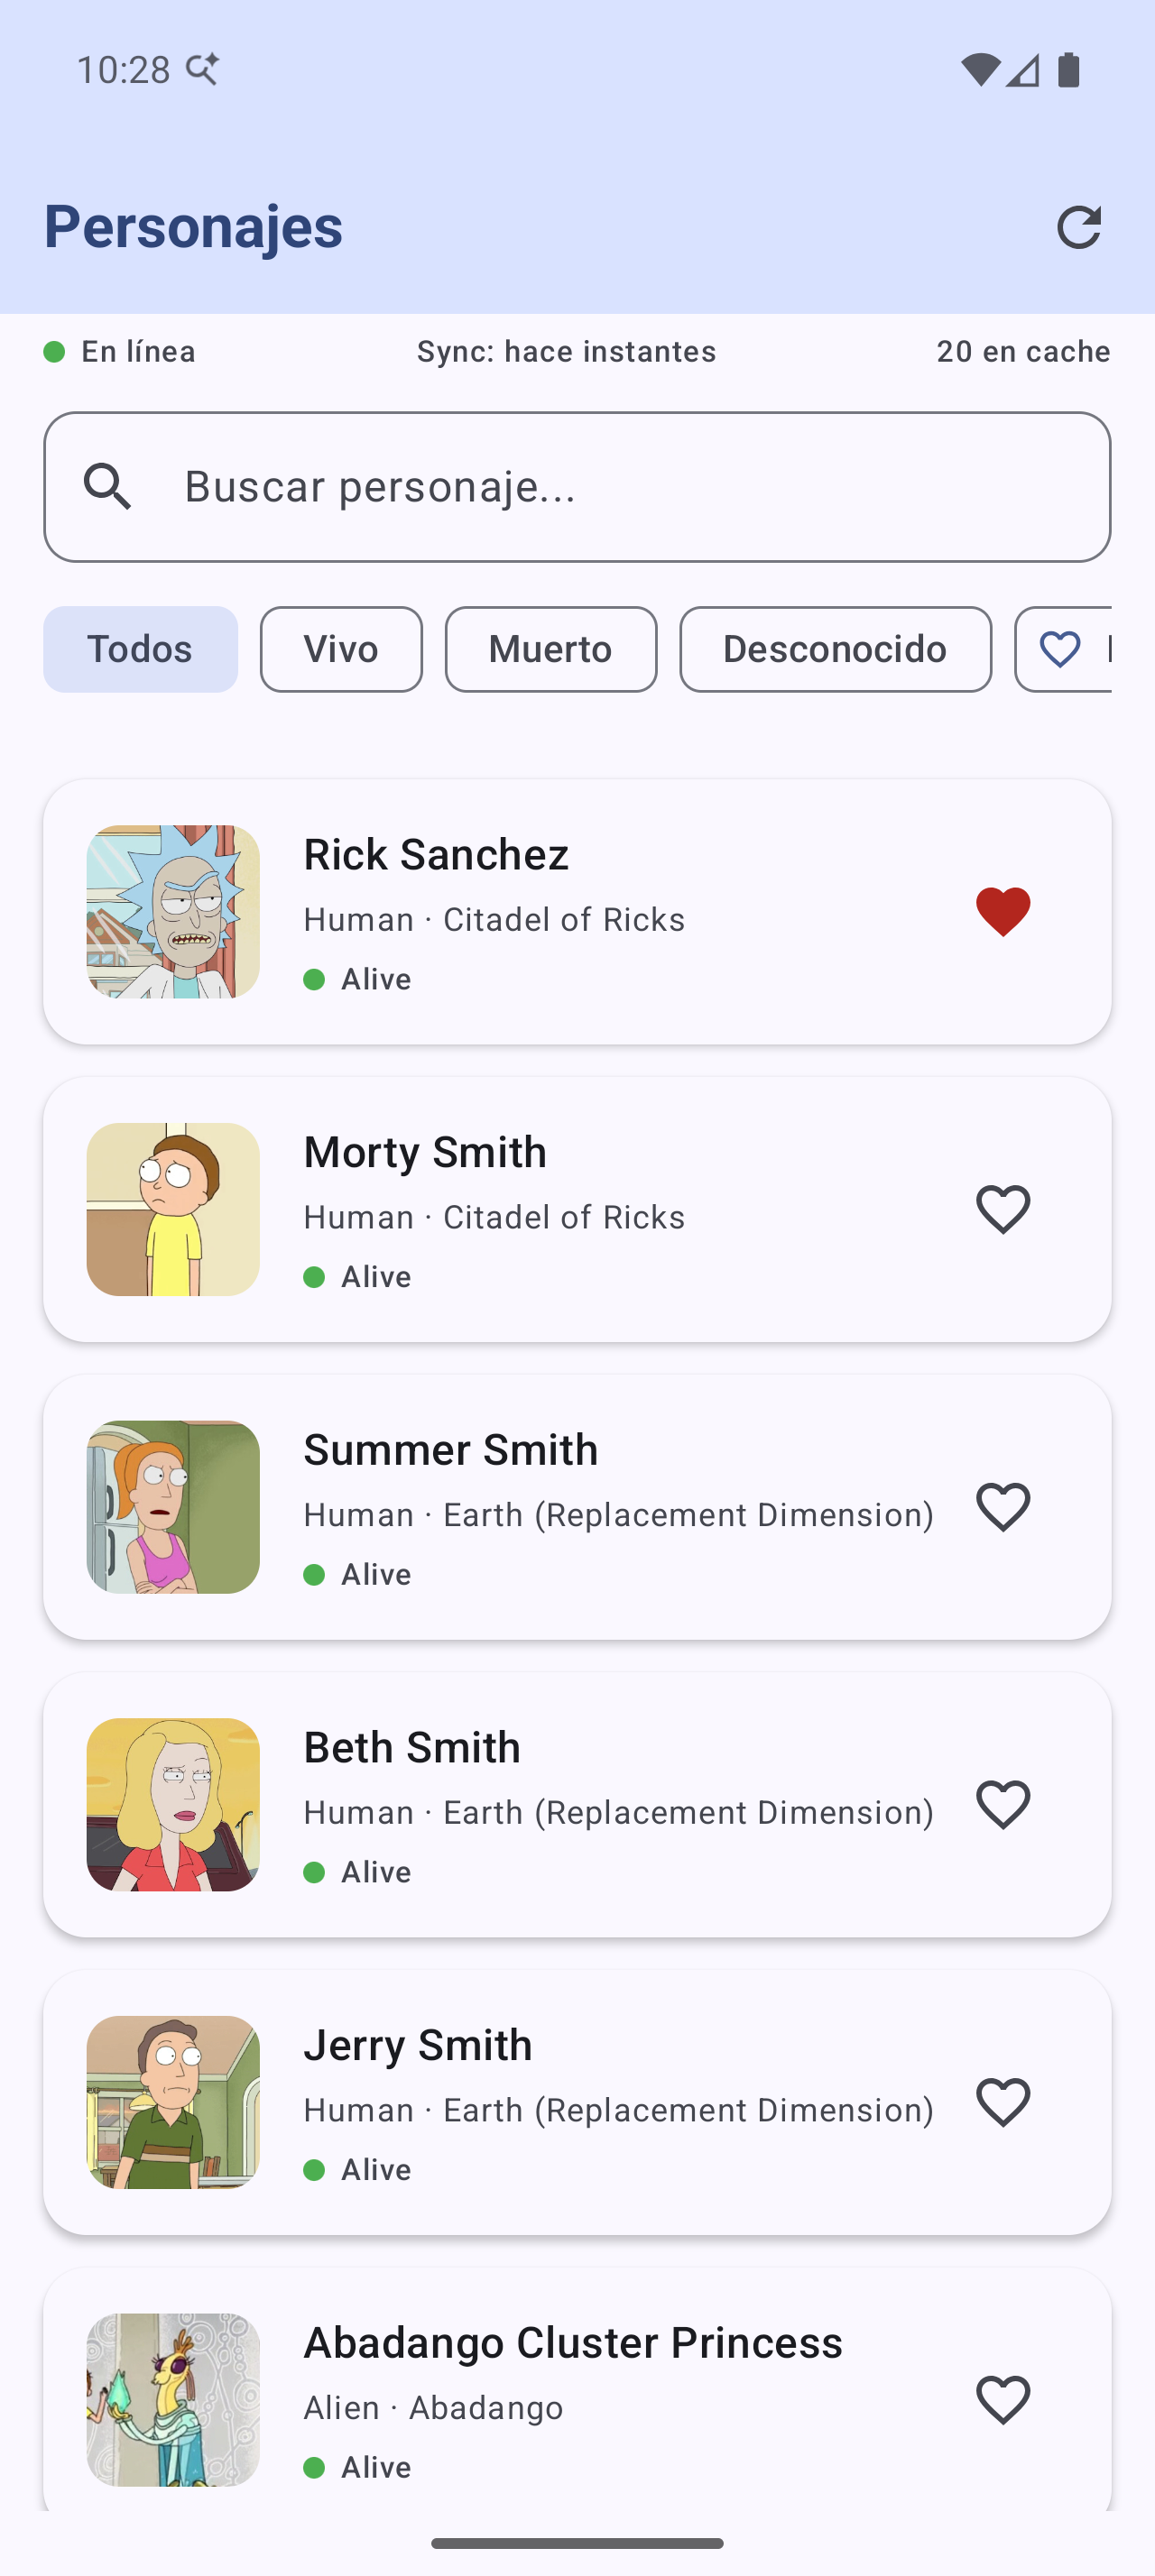
\includegraphics[width=\textwidth]{img/01_estado_online.png}
			\caption{Estado en línea: punto verde, "Sync: hace instantes", contador de cache.}
		\end{subfigure}
		\hfill
		\begin{subfigure}[t]{0.42\textwidth}
			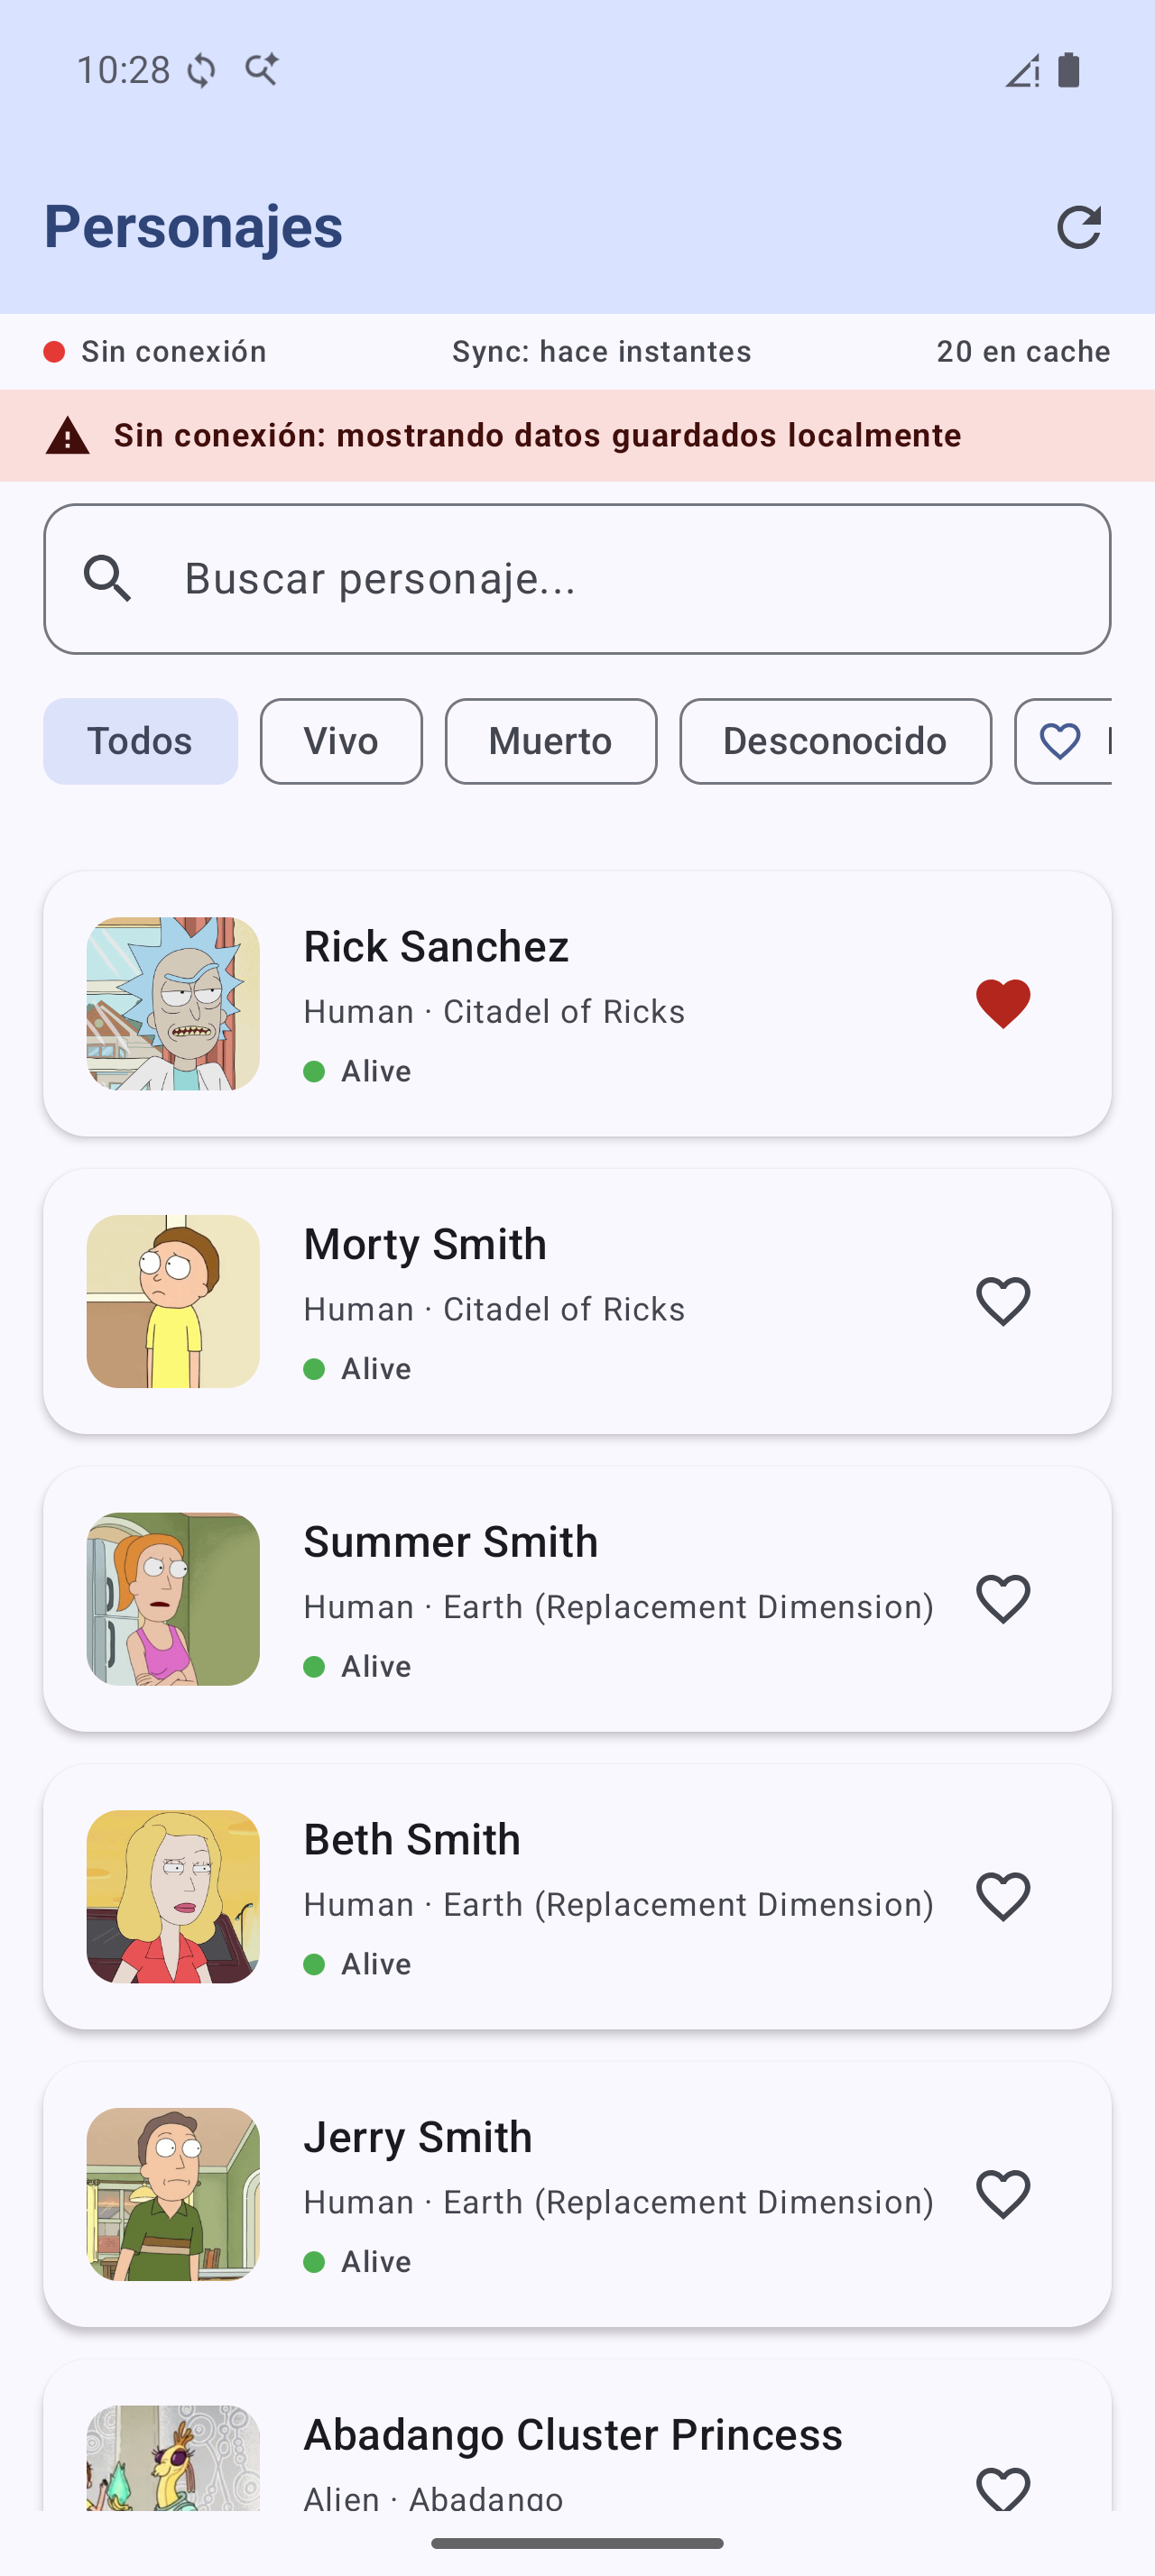
\includegraphics[width=\textwidth]{img/02_estado_offline.png}
			\caption{Estado sin conexión: punto rojo, banner de aviso, datos siguen visibles desde Room.}
		\end{subfigure}
		\caption{Objetivos a) y d): la app sigue mostrando datos consistentes con o sin conexión, y el panel de estado lo evidencia en tiempo real.}
	\end{figure}

	\begin{figure}[H]
		\centering
		\begin{subfigure}[t]{0.42\textwidth}
			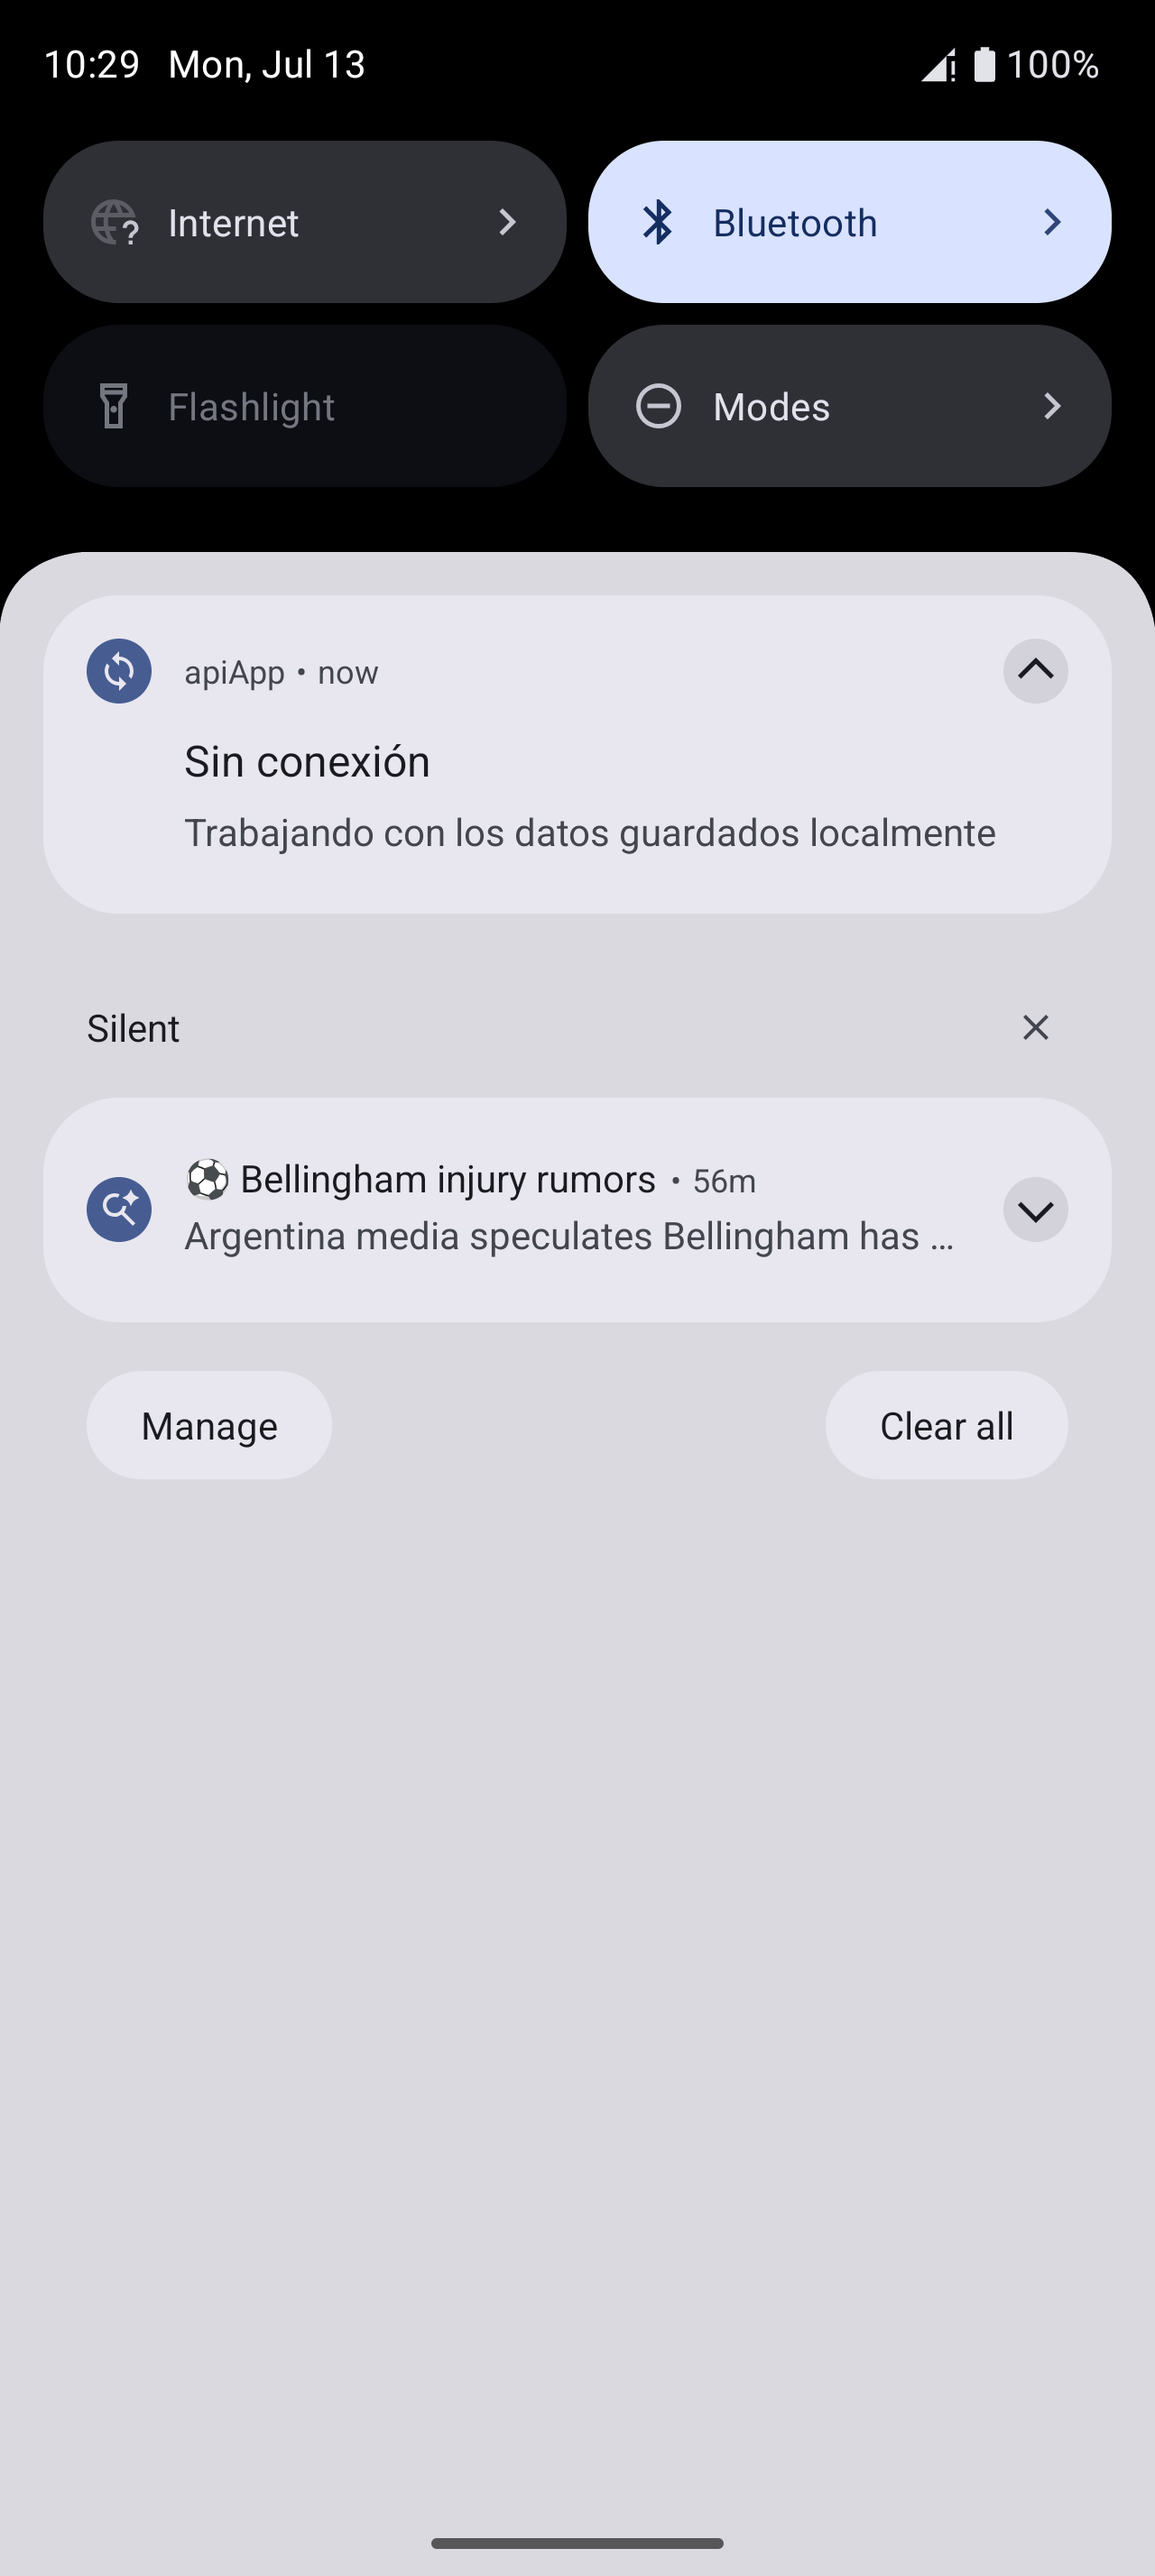
\includegraphics[width=\textwidth]{img/03_notificacion_desconexion.png}
			\caption{Notificación local al perder la conexión.}
		\end{subfigure}
		\hfill
		\begin{subfigure}[t]{0.42\textwidth}
			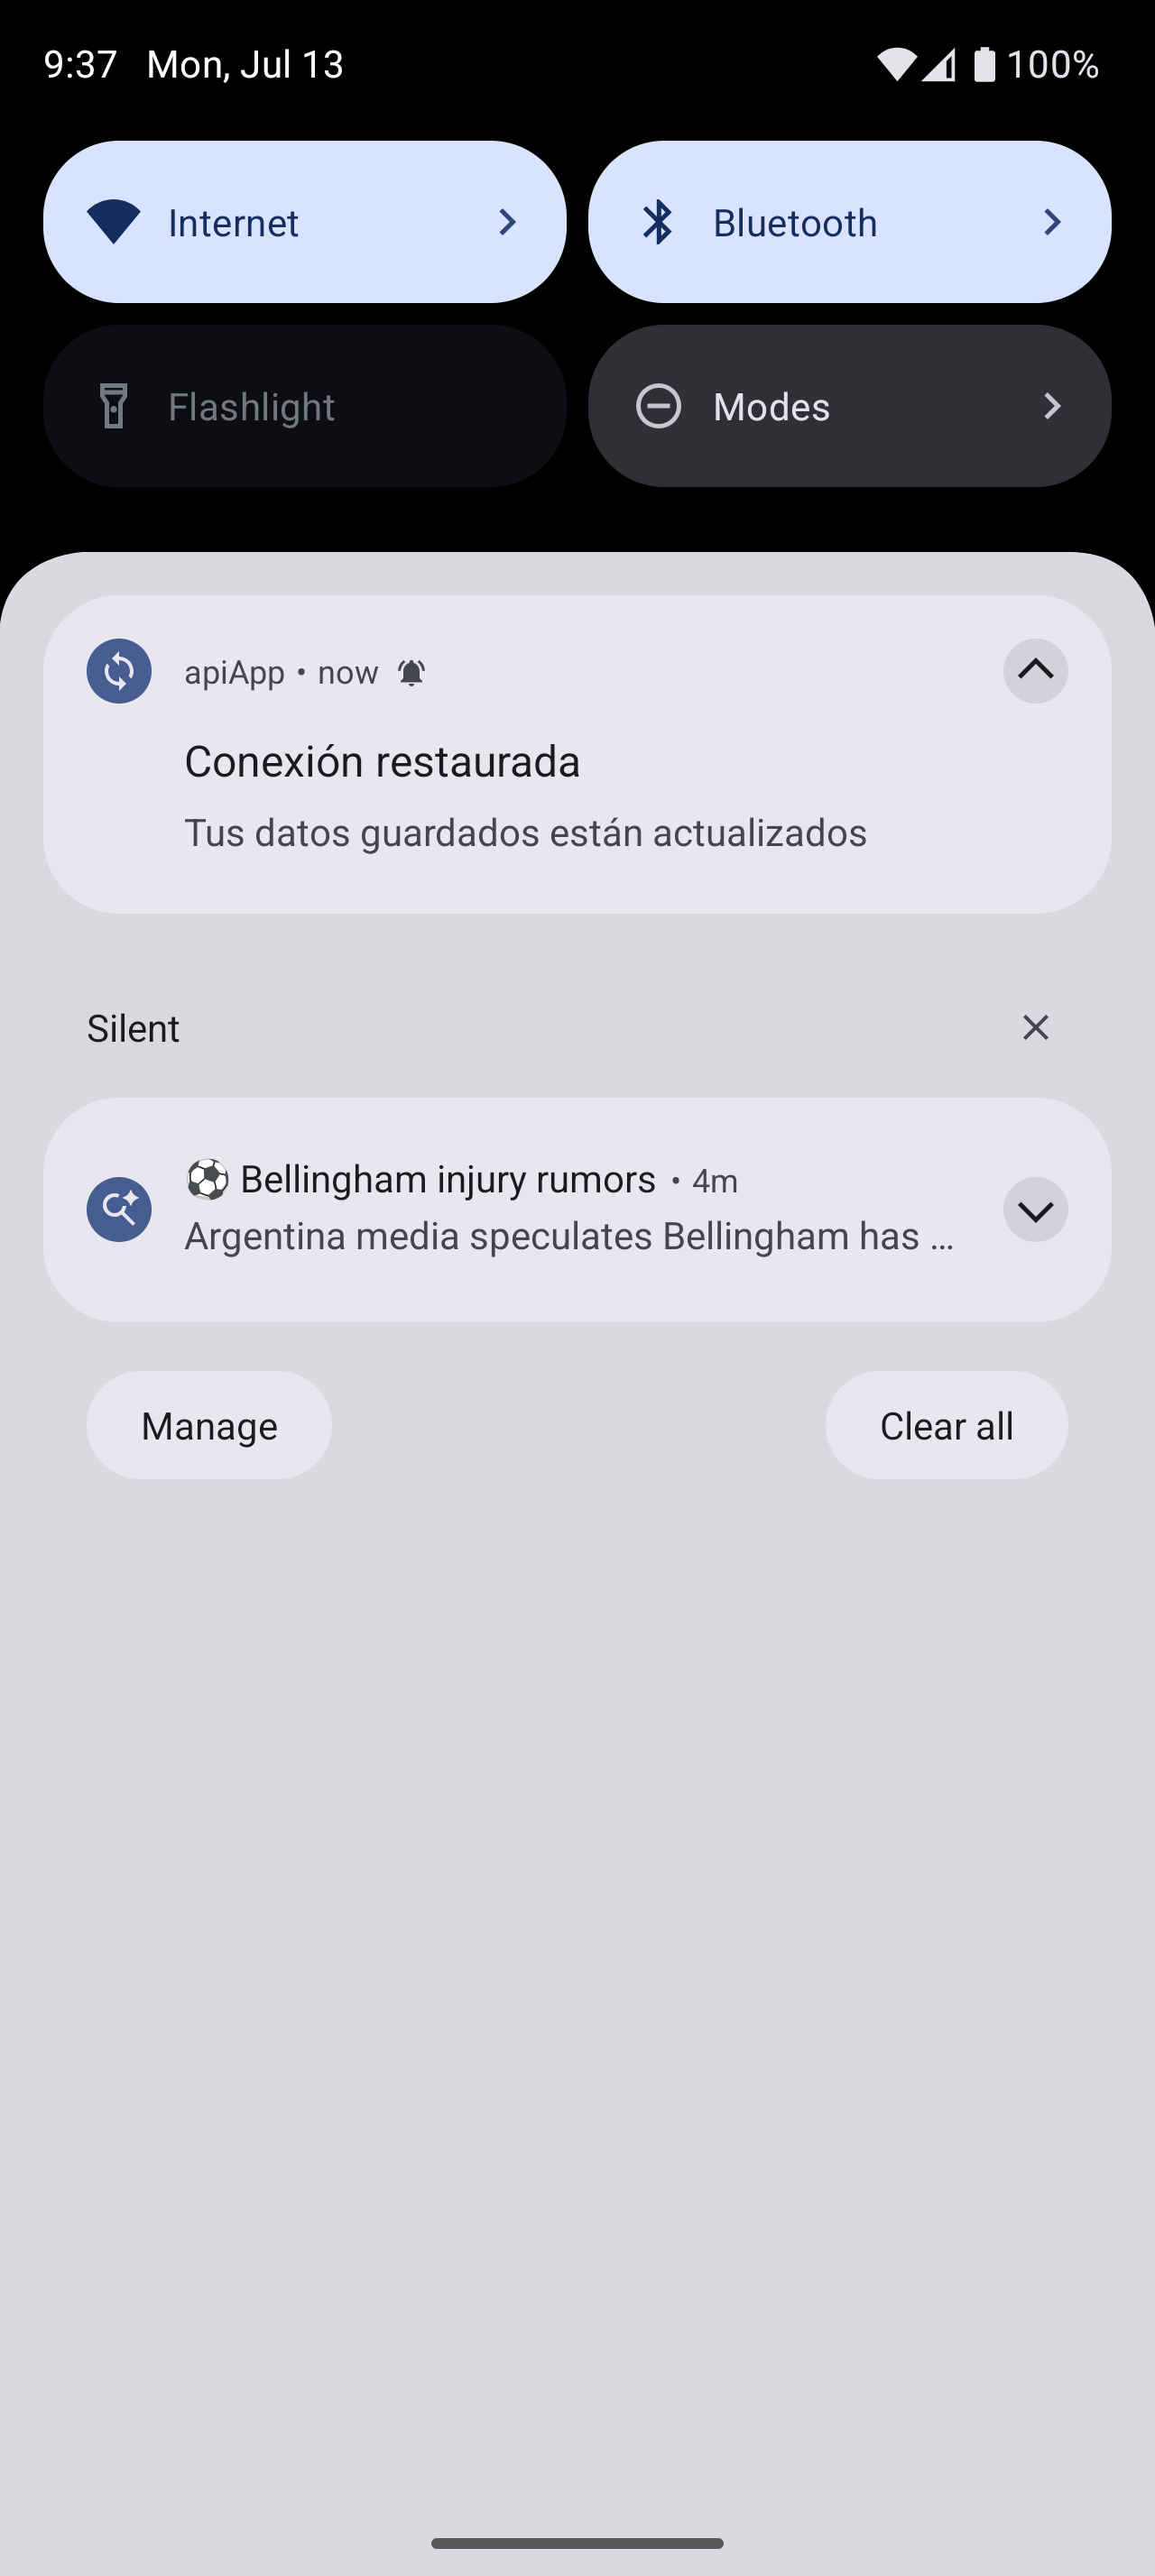
\includegraphics[width=\textwidth]{img/04_notificacion_reconexion.png}
			\caption{Notificación local al reconectar (dispara sincronización automática).}
		\end{subfigure}
		\caption{Notificaciones push locales reaccionando en ambos sentidos del cambio de conectividad, evidenciando el objetivo c).}
	\end{figure}

	\begin{figure}[H]
		\centering
		\begin{subfigure}[t]{0.42\textwidth}
			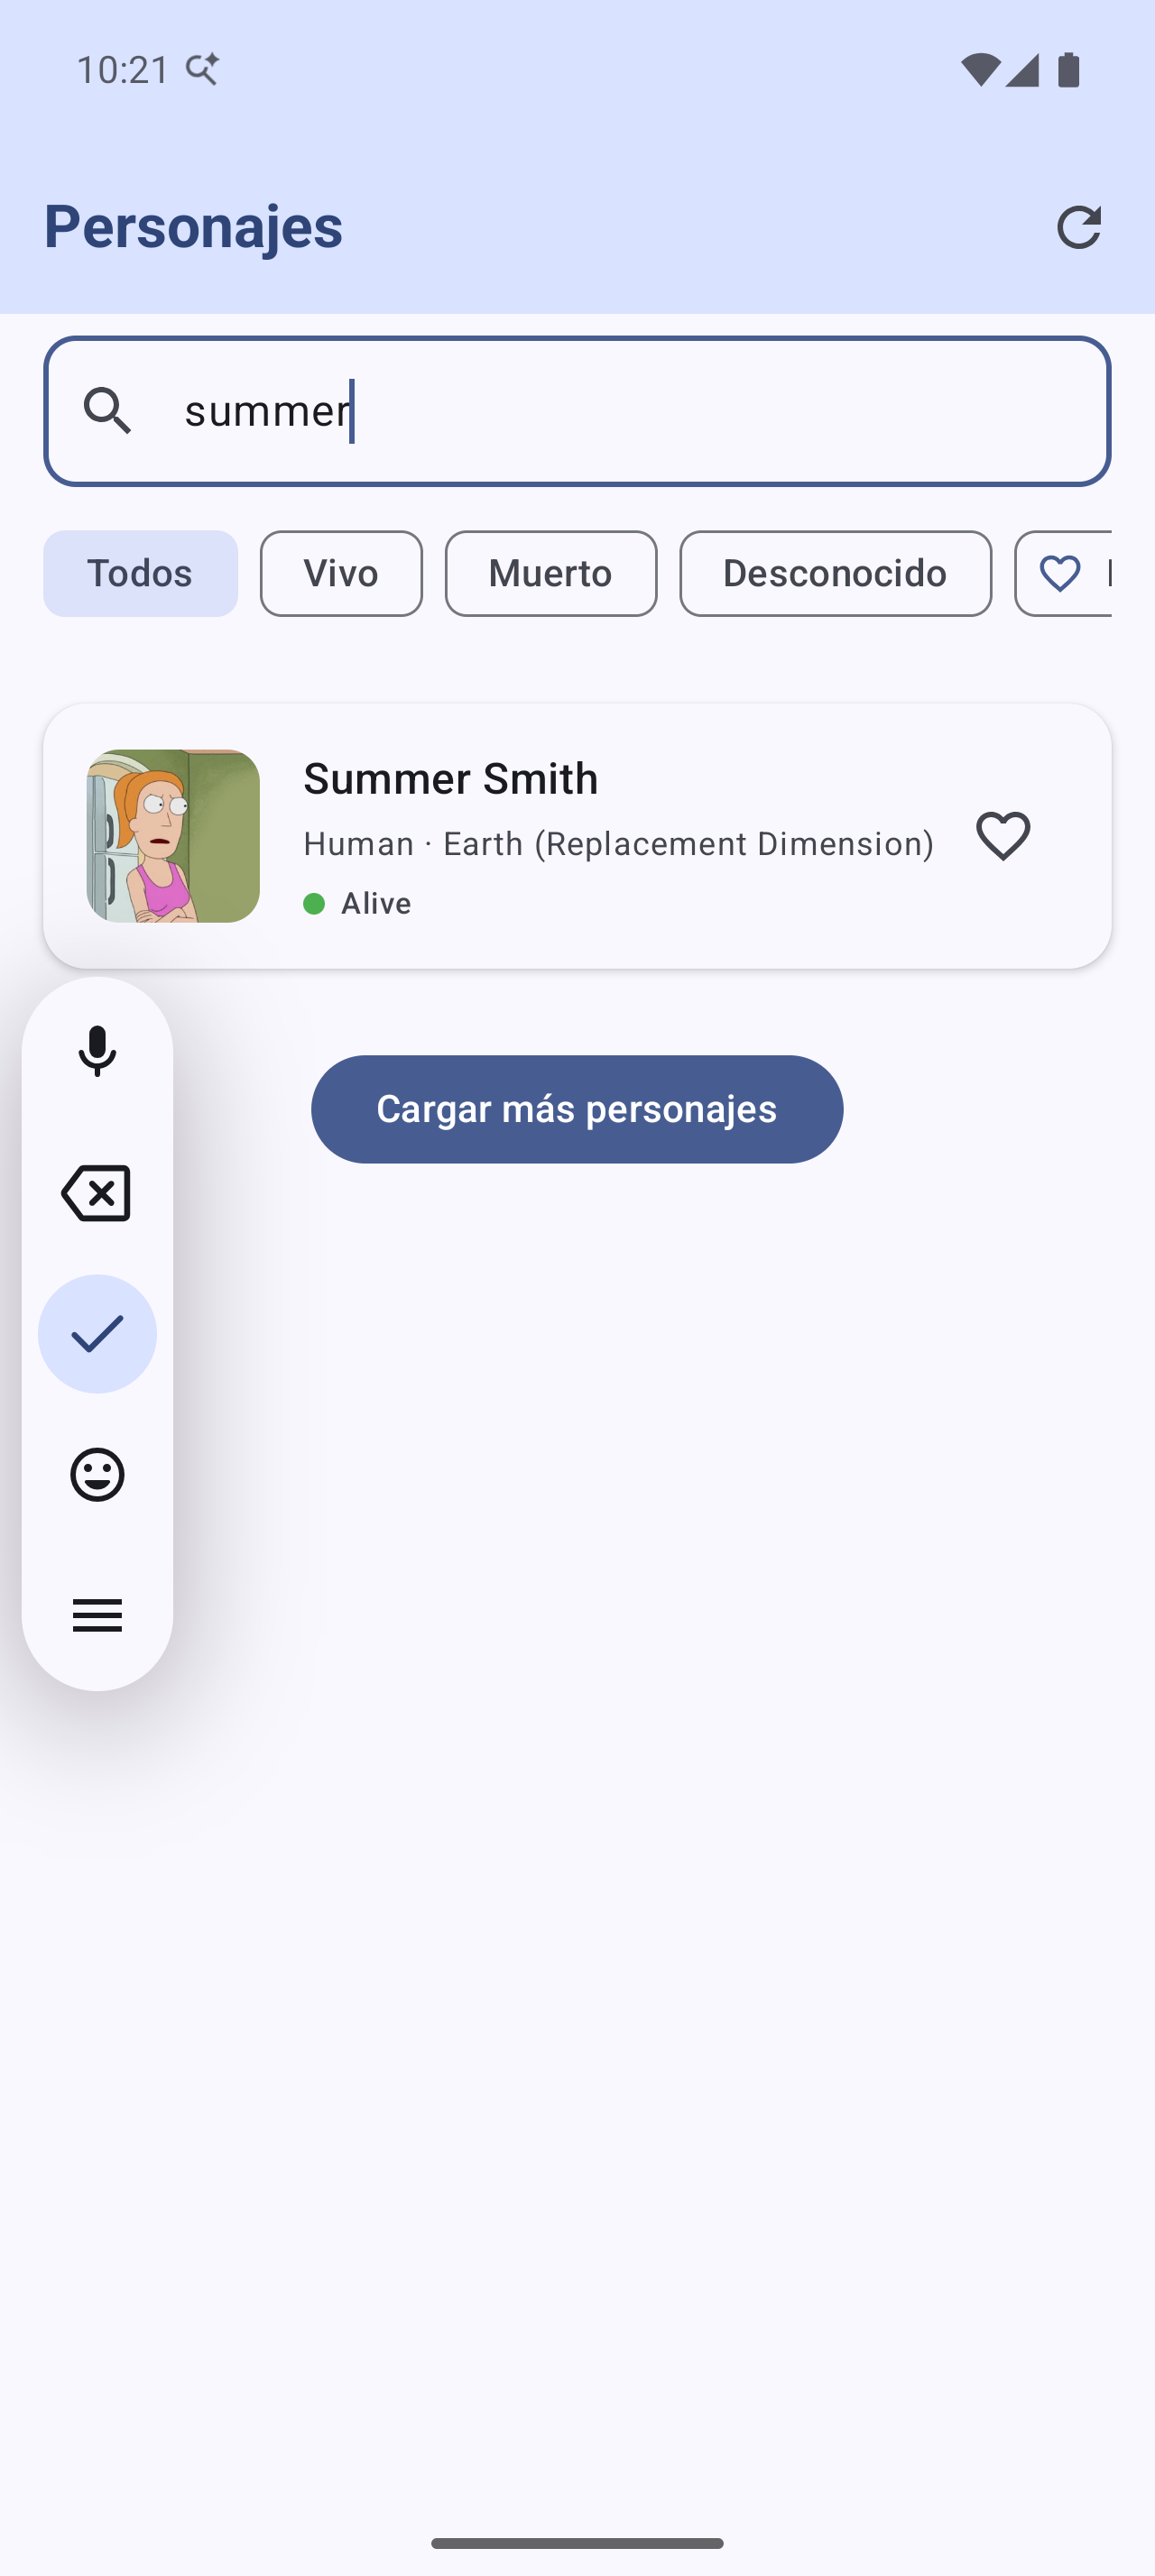
\includegraphics[width=\textwidth]{img/06_busqueda.png}
			\caption{Búsqueda en vivo sobre el cache local ("summer").}
		\end{subfigure}
		\hfill
		\begin{subfigure}[t]{0.42\textwidth}
			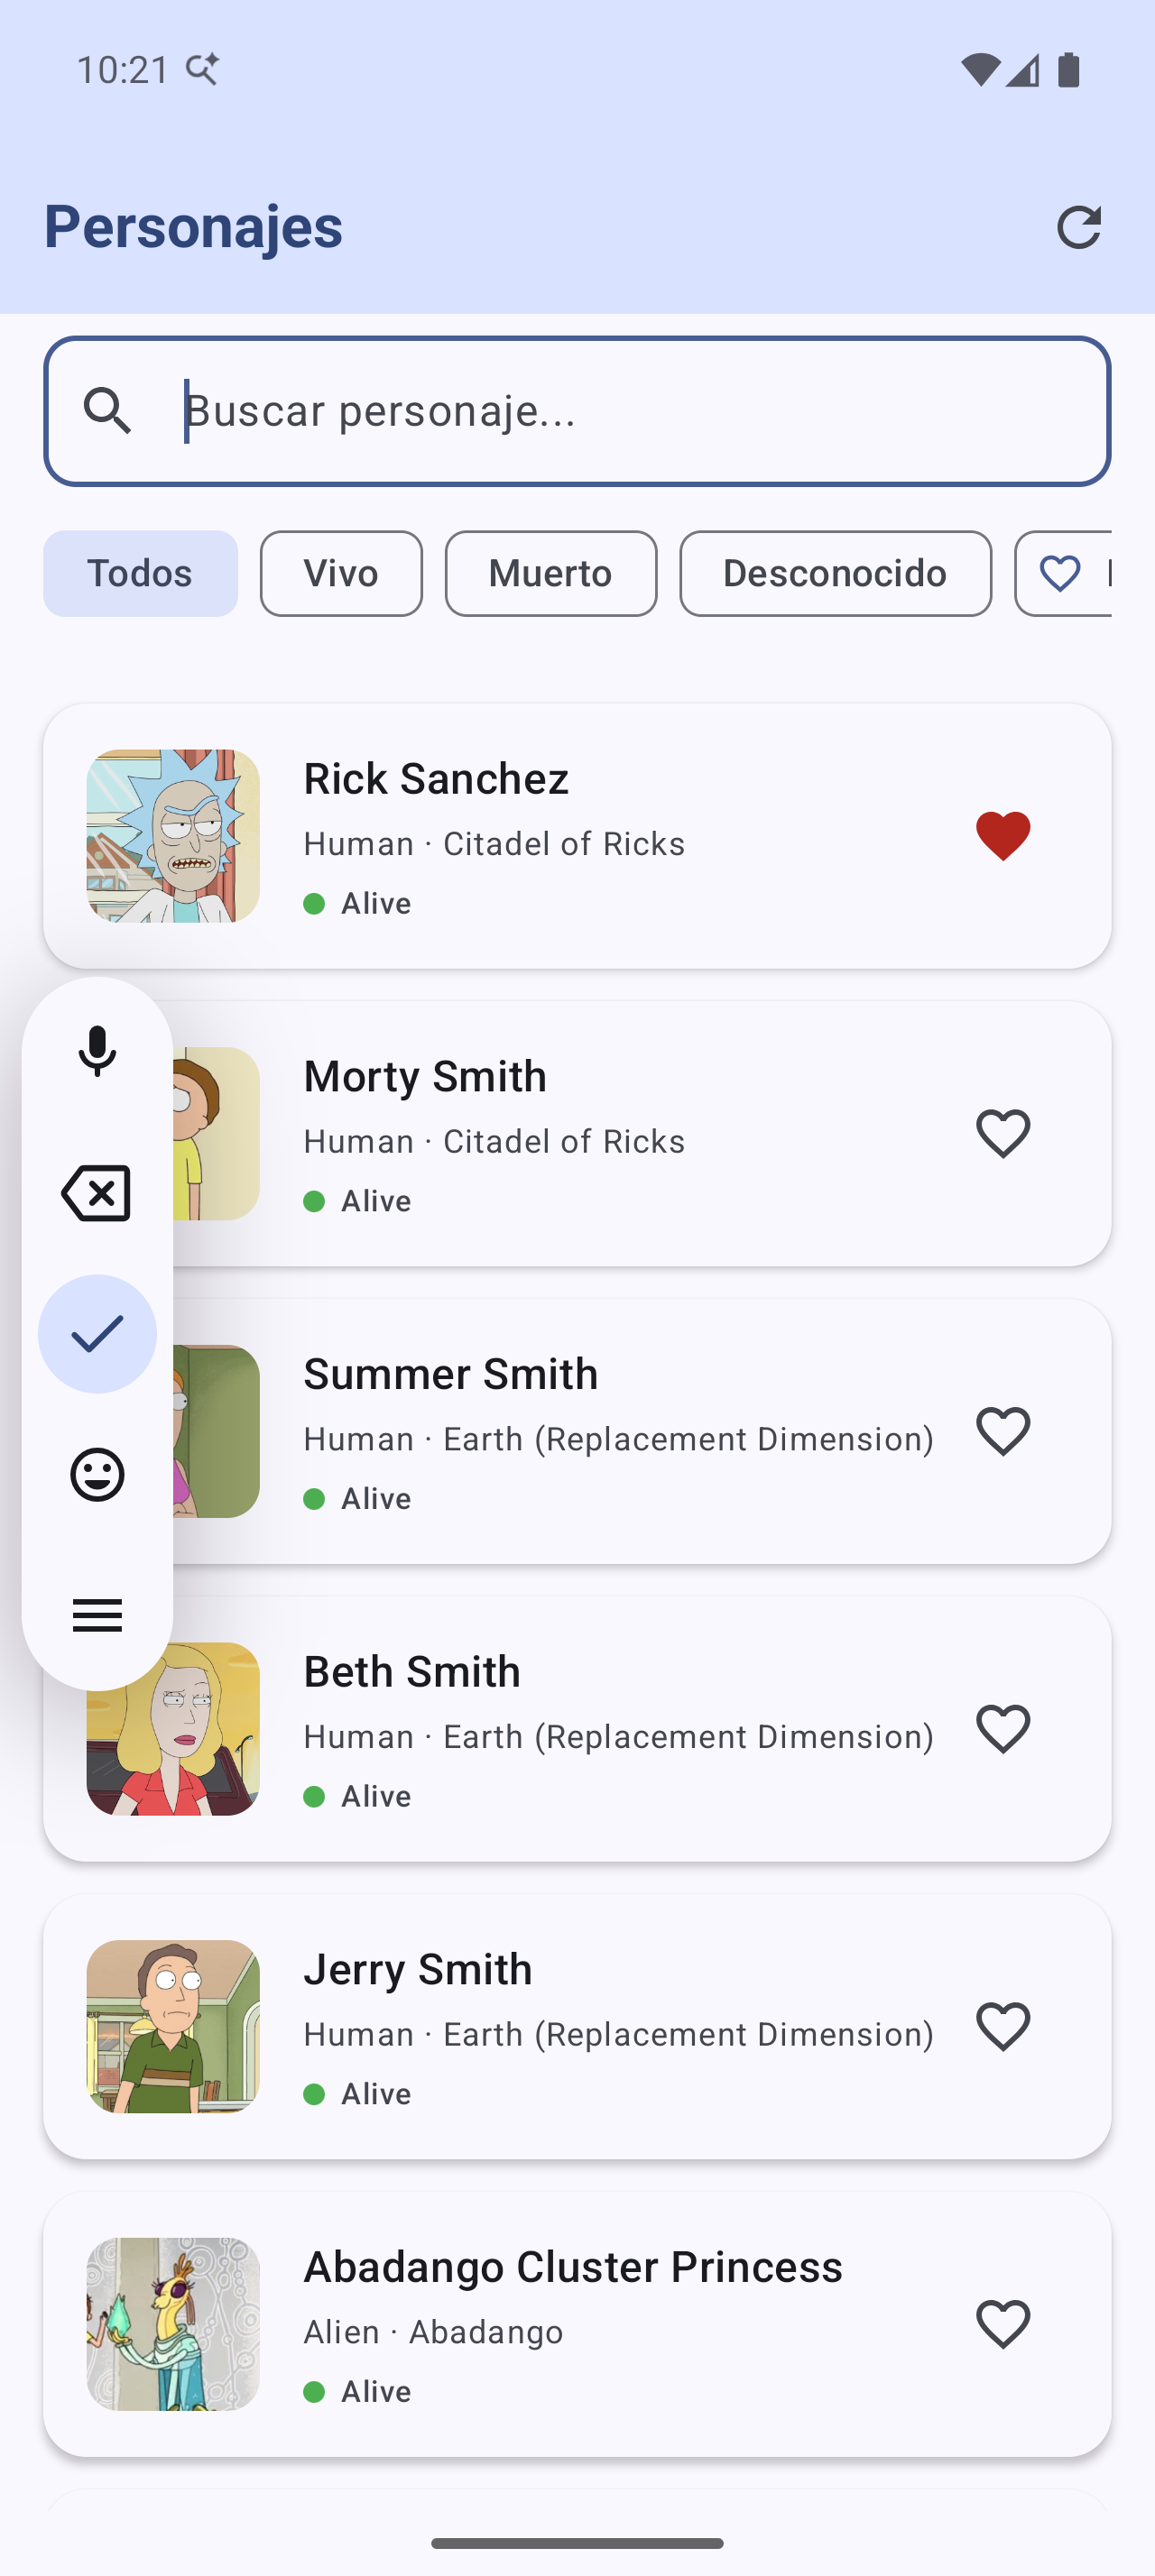
\includegraphics[width=\textwidth]{img/07_favoritos_filtro.png}
			\caption{Filtro de favoritos, persistido en Room.}
		\end{subfigure}
		\caption{Funcionalidad adicional construida sobre el mismo cache local: la consistencia UI-cache (objetivo d) se mantiene incluso al filtrar.}
	\end{figure}

	\begin{figure}[H]
		\centering
		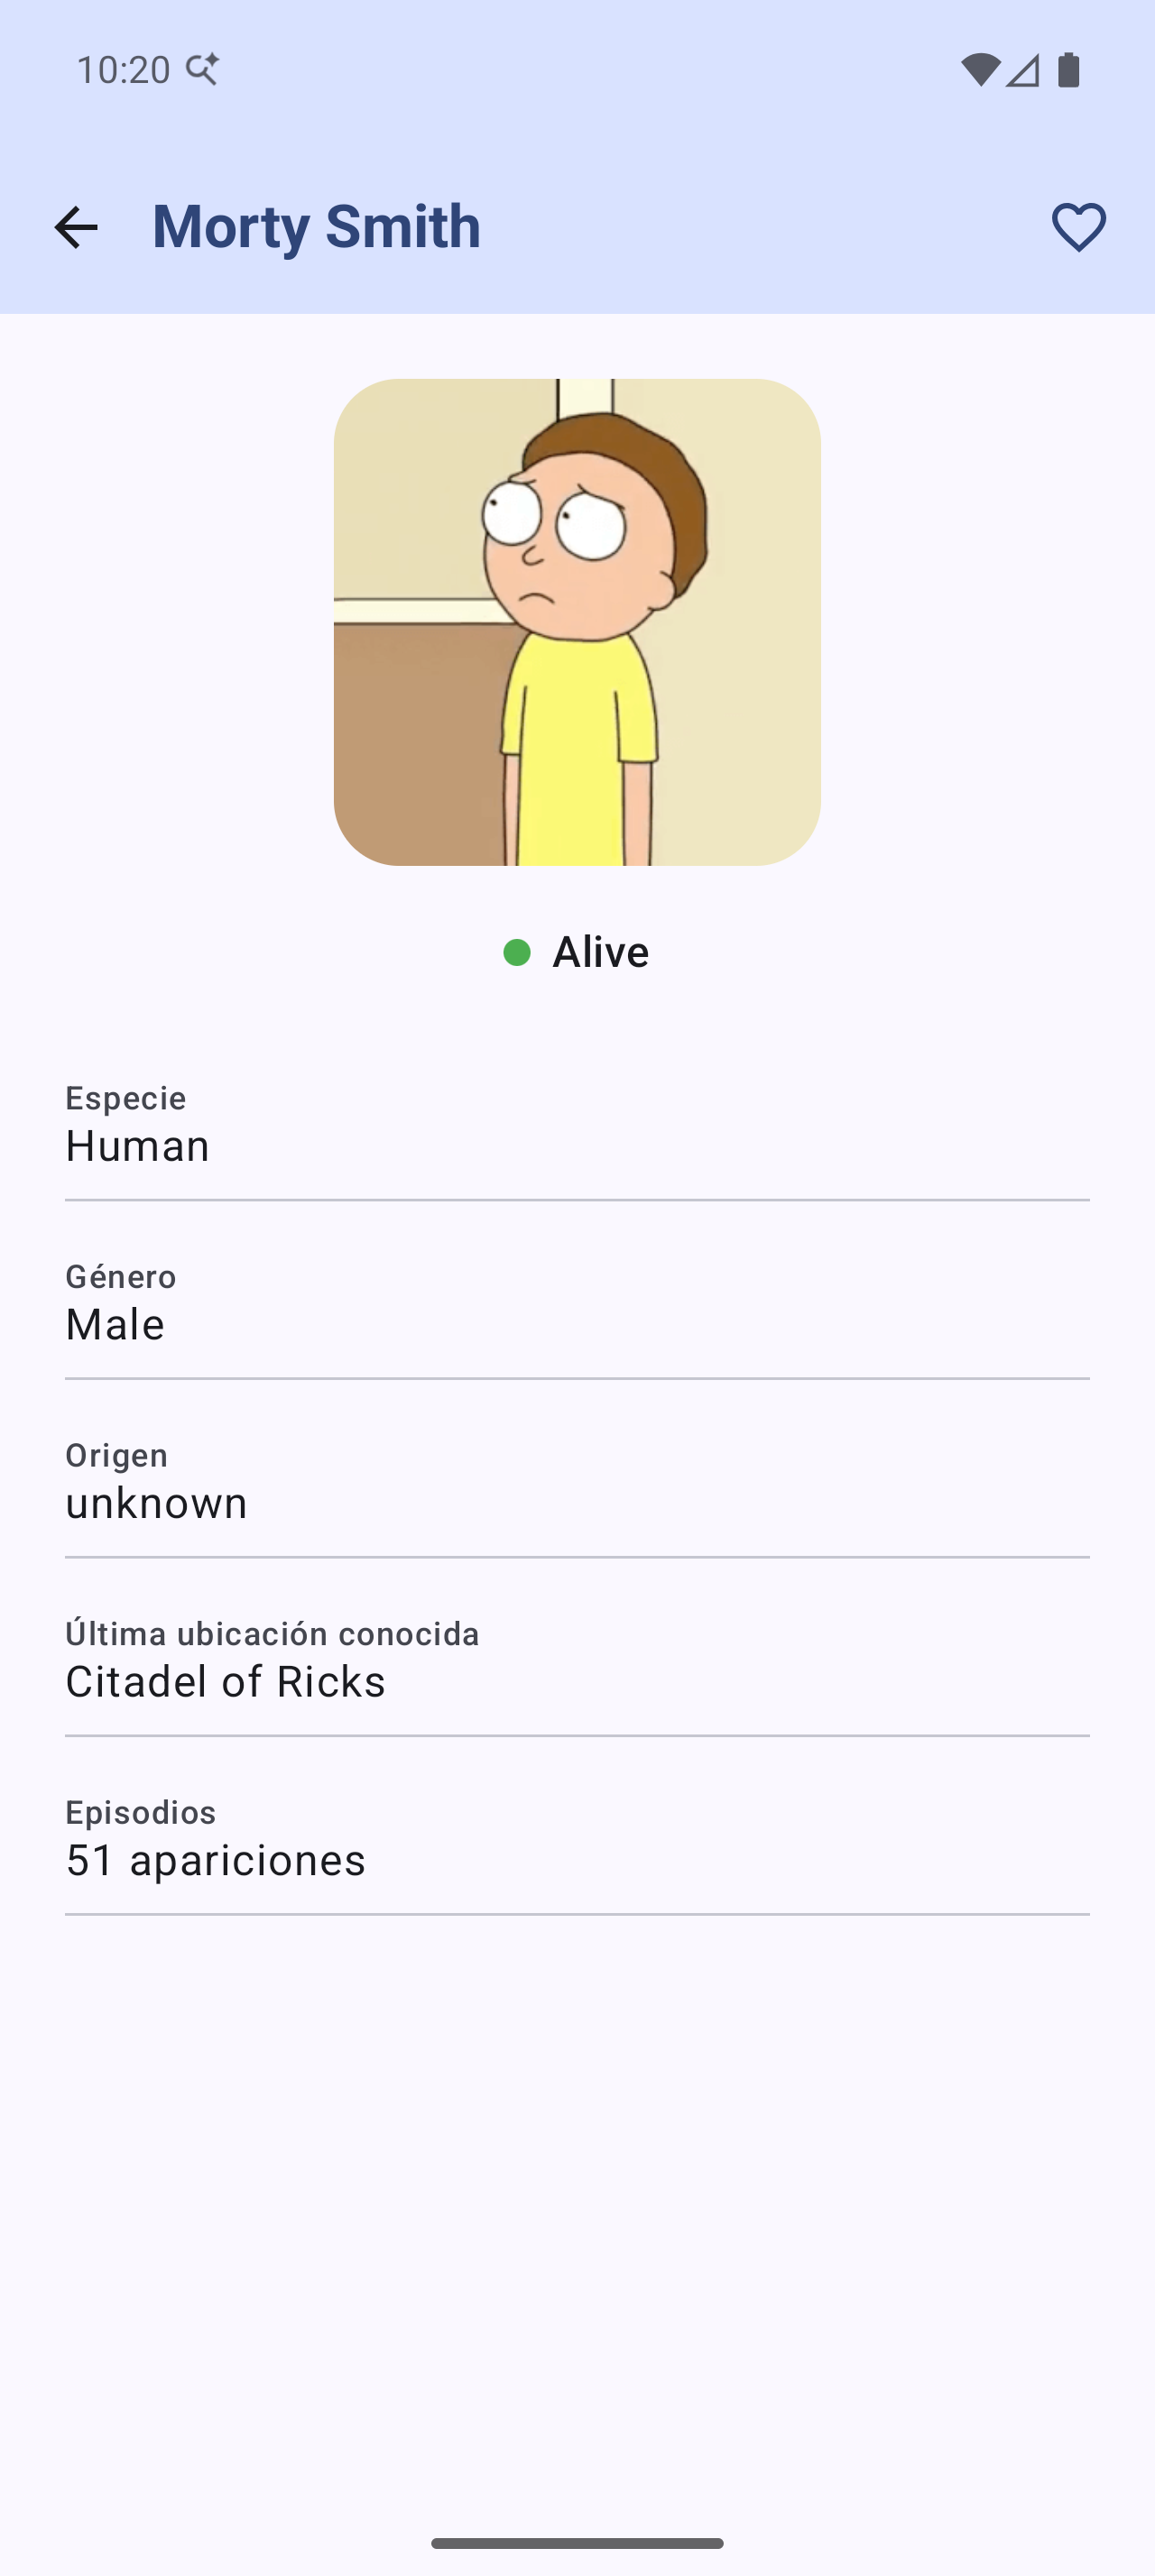
\includegraphics[width=0.4\textwidth]{img/05_pantalla_detalle.png}
		\caption{Pantalla de detalle de un personaje, alimentada íntegramente por Room (origen, ubicación, episodios).}
	\end{figure}

	Durante la ejecución se verificó además, revisando el \texttt{logcat} del emulador, que \texttt{WorkManager} inicializó correctamente el \texttt{SyncWorker} inyectado por Hilt (\texttt{Worker result SUCCESS for Work [...SyncWorker]}) y que ninguna de las pruebas -- incluyendo desconexión y reconexión repetidas, cambios de esquema de Room (migraciones), y navegación entre pantallas -- produjo una excepción no controlada (\texttt{FATAL EXCEPTION}).

	\section{Cuestionario}
	- Sin cuestionario -

	\clearpage
	\section{Conclusiones}
	\begin{itemize}
		\item Una arquitectura Offline-First bien aplicada no consiste en "guardar una copia de la respuesta de red", sino en invertir la fuente de verdad: la UI debe observar siempre la base de datos local (Room), y la red pasa a ser simplemente un mecanismo que alimenta esa base de datos. Este cambio de perspectiva es lo que permite que la app siga funcionando de forma consistente con o sin conexión.
		\item El pivote de API realizado (de \texttt{JSONPlaceholder} a Rick and Morty API) demostró que el diseño de la capa de red (Retrofit + DTOs + mappers) puede aislarse correctamente del resto de la arquitectura: el cambio de fuente de datos no afectó a Room, WorkManager, ni a la lógica de sincronización, que permanecieron intactos.
		\item Sincronizar automáticamente no es solo "volver a pedir los datos": hay que tener cuidado de no pisar estado local (como los favoritos) con cada actualización proveniente del servidor. Detectar y corregir este caso concreto durante las pruebas fue una de las lecciones más valiosas del laboratorio.
		\item Las notificaciones push "reales" (remotas, vía FCM) requieren necesariamente un backend propio capaz de emitirlas; en su ausencia, las notificaciones locales disparadas por eventos del propio dispositivo (cambios de conectividad, sincronización completada) son una alternativa legítima y totalmente funcional para informar al usuario, y comparten la misma infraestructura de canales y permisos que usaría un push remoto.
		\item Verificar el comportamiento en un emulador real (alternando modo avión, forzando reinicios en frío, revisando \texttt{logcat}) fue indispensable para detectar errores que no aparecen en una simple compilación exitosa, como el caso de los favoritos siendo sobrescritos silenciosamente durante la sincronización.
	\end{itemize}
	\clearpage

	\section{Referencias}
	\begin{itemize}
		\item \url{https://developer.android.com/training/data-storage/room}
		\item \url{https://developer.android.com/topic/libraries/architecture/workmanager}
		\item \url{https://developer.android.com/training/dependency-injection/hilt-android}
		\item \url{https://developer.android.com/develop/ui/views/notifications}
		\item \url{https://developer.android.com/reference/android/net/ConnectivityManager.NetworkCallback}
		\item \url{https://rickandmortyapi.com/documentation}
	\end{itemize}

\end{document}
